\documentclass[11pt]{article}
\usepackage{times}
\usepackage{amsmath,amsthm,amssymb,setspace,enumitem,epsfig,titlesec,verbatim,color,array,eurosym,multirow}
\usepackage[sort&compress,comma,round,numbers]{natbib}
\usepackage[footnotesize,bf]{caption}
\usepackage[margin=2.5cm, includefoot, footskip=30pt]{geometry}
\usepackage{standalone}
\usepackage{tikz}
\usepackage{subcaption}
\usepackage{hyperref}
\usepackage{tabularx}
\usepackage{booktabs}
\usepackage{blkarray}
\usepackage[ruled,vlined]{algorithm2e}
\smallskip % Erlaubt kleine Abstaende zwischen Paragraphen, falls es dem Seitenlayout hilft
\renewcommand{\baselinestretch}{1.3}
\newcommand{\R}{\mathbb{R}}

\newcommand{\todo}[1]{\textcolor{blue}{#1}}

\def\alld{\texttt{ALLD}}
\def\tft{\texttt{TFT}}
\def\gtft{\texttt{GTFT}}
\def\esm{electronic supplementary material}

%% Adding shortcut commands to refer to our figures %%
\newcommand{\FigBaseResults}{{\bf Fig.~1}} 
\newcommand{\FigDependenceParameters}{{\bf Fig.~2}} 
\newcommand{\FigHigherMemory}{{\bf Fig.~3}}


\titleformat{\section}{\sffamily \fontsize{12}{14}\bfseries}{\thesection}{1em}{}
\titleformat{\subsection}{\sffamily
\fontsize{11.5}{11.5}\bfseries}{\thesubsection}{1em}{}

\usepackage{tikz}
\usetikzlibrary{arrows}

\tikzset{treenode/.style = {align=center, inner sep=0pt, text centered,
  font=\sffamily}, arn_n/.style = {treenode, circle, white,
  font=\sffamily\bfseries, draw=black, inner sep=-6pt, fill=black, text
  width=1.5em},% arbre rouge noir, noeud noir
  arn_r/.style = {treenode, circle, red, text width=1.5em, very thick, inner
    sep=4pt},% arbre rouge noir, noeud rouge
  arn_x/.style = {treenode, rectangle, draw=black, minimum width=0.5em, minimum
    height=0.5em}% arbre rouge noir, nil
}

\newtheoremstyle{plainCl1}% name
{9pt}%      Space above, empty = 'usual value'
{9pt}%      Space below
{\it}% 	   Body font
{}%         Indent amount (empty = no indent, \parindent = para indent)
{\bfseries}% Thm head font
{.}%        Punctuation after thm head
{0.2cm}% Space after thm head: \newline = linebreak
{}%         Thm head spec

\newtheoremstyle{plainCl2}% name
{9pt}%      Space above, empty = 'usual value'
{9pt}%      Space below
{\it}% 	   Body font
{}%         Indent amount (empty = no indent, \parindent = para indent)
{\bfseries}% Thm head font
{$'$.}%        Punctuation after thm head
{0.2cm}% Space after thm head: \newline = linebreak
{}%         Thm head spec


\theoremstyle{plainCl1}
\newtheorem{Claim}{Claim}
\newtheorem{Thm}{Theorem}
\newtheorem{Prop}{Proposition}
\newtheorem*{Lem}{Lemma}
\newtheorem{Cor}{Corollary}
\newtheorem*{Def}{Definition}

\theoremstyle{plainCl2}
\newtheorem{Claim2}{Claim}




\title{\bf  \sffamily \Large Evolution of reciprocity %among individuals\\ 
with limited payoff memory\\}
\date{}
\author{\parbox[c]{16cm}{\centering \onehalfspacing 
Nikoleta E. Glynatsi$^1$,  Alex McAvoy$^{2,3}$, Christian Hilbe$^1$\\ \quad \\
$^{\rm 1}$Max Planck Research Group on the Dynamics of Social Behavior,\\ Max Planck Institute for Evolutionary Biology, Pl\"{o}n, Germany \\
$^{\rm 2}$School of Data Science and Society, University of North Carolina at Chapel Hill,\\ Chapel Hill, NC 27599 \\
$^{\rm 3}$Department of Mathematics, University of North Carolina at Chapel Hill,\\ Chapel Hill, NC 27599}}

\begin{document}
\maketitle


\begin{abstract}
\noindent
Direct reciprocity can explain the evolution of cooperative behaviors in repeated interactions. 
According to this literature, individuals should naturally learn to adopt conditionally cooperative strategies if they have multiple encounters with their interaction partner. 
Corresponding models have greatly facilitated our understanding of cooperation, yet they often make strong assumptions on how individuals remember and process payoff information. 
For example, when strategies are updated through social learning, it is commonly assumed that individuals compare their respective average payoffs.  
This would require them to compute (or remember) their payoffs against everyone else in the population.
To understand how more realistic constraints influence direct reciprocity, we consider the evolution of conditional behaviors when individuals learn based on more recent experiences.
Even in the most extreme case that they only take into account their very last interaction, we find that cooperation can still evolve. 
However, such individuals adopt less generous strategies, and they tend to cooperate less often than in the classical setup with expected payoffs. 
Interestingly, once individuals remember the payoffs of two or three recent interactions, cooperation rates quickly approach the classical limit. 
These findings contribute to a literature that explores which kind of cognitive capabilities are required for reciprocal cooperation. 
While our results suggest that some rudimentary form of payoff memory is necessary, it already suffices to remember a few interactions.
\end{abstract}

~\\
{\it Keywords:} Evolution of cooperation; direct reciprocity; repeated prisoner's dilemma; social learning; evolutionary dynamics



\clearpage
\newpage


%%%%%%%%%
%%  INTRO  %%
%%%%%%%%%

\section{Introduction}

%% INTRO: General introduction to evolutionary game theory and cognitive constrains

Evolutionary game theory describes the dynamics of populations when an individual's fitness depends on the traits or strategies of other population members~\cite{hofbauer1998evolutionary, nowak:Nature:2004, hauert2005game,Traulsen:PhilTrans:2022}.  
This theory can be used to describe the dynamics of animal conflict~\citep{maynard-smith:Nature:1973}, cancer cells~\citep{Stein:PTRS:2023}, and of cooperation~\citep{nowak:Science:2006}. 
Respective models translate strategic interactions into games~\cite{smith1982evolution}. 
These games specify how individuals (players) interact, which strategies individuals can choose, and what fitness consequences (or payoffs) the different strategies have. 
In addition, these models also specify the mode by which successful strategies spread over time. 
In models of biological evolution, individuals with a high fitness produce more offspring; in models of cultural evolution, such individuals are imitated more often. 
Although biological and cultural evolution are sometimes treated as equivalent, there can be important differences~\citep{Wu2015,Smolla:PTRS:2021}. 
For example, models of biological evolution do not require individuals to have any particular cognitive abilities.
Here, it is the evolutionary process itself that biases the population towards strategies with higher fitness. 
In contrast, in models of cultural evolution, individuals need to be aware of the different strategies present in the population, and they need to identify those strategies with a higher payoff. 
As a consequence, evolutionary outcomes may depend on how easily different behaviors can be learned~\citep{Chatterjee:JTB:2012}, and on how easy payoff comparisons are. 

%% INTRO: Literature on direct reciprocity and why social learning of strategies is hard

These difficulties to learn strategies by social imitation are particularly pronounced in models of direct reciprocity. 
This literature follows Trivers' insight that individuals have more of an incentive to cooperate in social dilemmas when they interact repeatedly~\citep{trivers1971evolution}. 
In repeated interactions, individuals can condition their behavior on their past experiences with their interaction partner. 
They may use strategies such as Tit-for-Tat~\citep{rapoport:book:1965,axelrod1981evolution} or Generous Tit-for-Tat~\citep{molander:jcr:1985,Nowak1992tit} to preferentially cooperate with other cooperators. 
Such conditional strategies approximate human behavior fairly well~\citep{fischbacher:EconL:2001,Rand:TCS:2013,DalBo:AER:2019,Rossetti:ETH:2023} and they have also been documented in several other species~\citep{Carter:PRSB:2013,Schweinfurth:AnBehav:2019,Voelkl:PNAS:2015} -- although direct reciprocity is generally more difficult to demonstrate in animals~\citep{CluttonBrock:Nature:2009,Silk:CurrentBiology:2013,taborsky:CurrentBiology:2013}.
However, at the outset, it is not clear how easy it is to {\it learn} reciprocal strategies by social imitation. 
As one obstacle, even if others' strategies are perfectly observable, individuals might find it difficult to identify which ones have the highest payoff. 
After all, the payoff of a strategy of direct reciprocity is not determined by the outcome of any single round.
Rather, it is determined by how well this strategy fares over an entire sequence of rounds, against many different population members. 
In practice, such information might be both difficult to obtain and to process. 

%% INTRO: Gap in the literature and what  question we wish to address. 

Most models of direct reciprocity abstract from these difficulties~\citep{brauchli:JTB:1999,brandt:JTB:2006,ohtsuki:JTB:2007b,szolnoki:pre:2009b,imhof2010stochastic,van-segbroeck:prl:2012,grujic:jtb:2012,Martinez2012,stewart:pnas:2013,pinheiro:PLoSCB:2014,stewart:games:2015,Baek2016,McAvoy:ProcA:2019,glynatsi:SCR:2020,Schmid:PlosCB:2022,Murase:SciRep:2022}. 
They just assume individuals can easily copy the strategies of others. 
Similarly, they just assume that updating decisions are based on the strategies' average (or expected) payoffs, which are based on all rounds and all interactions. 
These assumptions create a curious inconsistency in how models represent an individual's cognitive abilities. 
On the one hand, when playing the game, individuals are often assumed to have restricted memory. 
Respective studies typically assume that individuals make their decisions each round based on the outcome of the last round only~\citep[with only a few exceptions, see Refs.][]{Hauert1997,van-veelen:PNAS:2012,Stewart2016,Li:NatCS:2022,Murase:PLoSCompBio:2023a}. 
Yet when learning new strategies, individuals are assumed to remember (or compute) each others' precise average payoff across many rounds and many interaction partners. 
Herein, we wish to explore whether this latter assumption is actually necessary for the evolution of reciprocity through social imitation. 
We ask whether individuals can learn to adopt reciprocal strategies even when learning is based on payoff information from a limited number of rounds. 


%% INTRO: Basic description of our model and our findings 

To explore that question, we theoretically study imitation dynamics in the repeated prisoner's dilemma, using two extreme scenarios. 
The first scenario is the usual modeling approach. 
Here, individuals update their strategies based on their expected payoffs. 
We contrast this model with an alternative scenario where individuals update their strategies based on the very
last (one-shot) payoff they obtained. 
We find that individuals with limited payoff memory tend to adopt less generous strategies. 
Yet moderate levels of cooperation can still evolve. 
Moreover, as we increase the individuals' payoff memory to include the last two or three one-shot payoffs, cooperation rates quickly approach the rates observed in the classical baseline case. 

%% INTRO: Summary and conclusions

Overall, these findings suggest that while memory is important, already minimal payoff information may suffice for the evolution of direct reciprocity based on social learning. 
They also suggest that the classical model of reciprocity (based on expected payoffs) can often be interpreted as a useful approximation to more realistic models that include cognitive constraints. 



%%%%%%%%%
%% MODEL  %%
%%%%%%%%%


\section{Model and Methods}\label{section:model}

%% MODEL: Basic intro

To explore the impact of limited payoff memory, we adapt existing models of the evolution of direct reciprocity through social learning. 
These models involve two different time scales. 
The short time scale describes the game dynamics. 
Here, individuals with fixed strategies are randomly matched to interact with each other in repeated social dilemmas. 
The long time scale describes the evolutionary dynamics. 
Here, individuals can update their repeated-game strategies based on the payoffs they yield. 
In the following, we introduce the basic setup of our model; all details and derivations are described in the \esm.\\

%% MODEL: (Repeated) donation game

\noindent
{\bf Description of the game dynamics.} We consider a well-mixed population consisting of $N$~players.
Players are randomly matched in pairs to participate in a repeated donation game~\citep{sigmund2010calculus}.
Each round, players can either cooperate (\(C\)) or defect (\(D\)). 
By cooperating, a player provides a benefit \(b\) to the other player at their own cost \(c\), with \(0 \!<\! c \!<\! b\). 
Thus, the players' payoffs in a single round are given by the matrix
\begin{align}
\bordermatrix{%
	& C & D \cr
C &\ b-c &\ -c\  \cr
D &\ b &\ 0\ \cr
} .
\end{align}
In particular, payoffs take the form of a prisoner's dilemma:
Mutual cooperation yields a better payoff than mutual defection ($b\!-\!c\!>\!0$), but each player individually prefers to defect independent of the co-player's action ($b\!>\!b\!-\!c$ and $0\!>\!-c$). 
To incorporate that individuals interact repeatedly, we assume that after each round, there is a constant continuation probability $\delta$ of interacting for another round. 
For $\delta\!=\!0$, we recover the case of a conventional (one-shot) prisoner's dilemma. 
Here, mutual defection is the only equilibrium. 
As $\delta$ increases, the game turns into a repeated game. Here, additional equilibria emerge, with some of them allowing for full cooperation~\citep{friedman:RES:1971,Akin:chapter:2016,hilbe:GEB:2015,stewart:pnas:2014}. 


%% MODEL: Reactive strategies

In a one-shot donation game, players can only choose among two pure strategies (they can either cooperate or defect).
In the repeated game, strategies become arbitrarily complex. 
Here, strategies are contingent rules, telling players what to do depending on the outcome of all their previous interactions. 
For simplicity, in the following we assume individuals use {\it reactive strategies}~\citep{Nowak1992tit}. 
A reactive strategy only depends on the other player's action in the previous round. 
Such strategies can be written as a three-dimensional tuple \(\mathbf{s}=(y, p,q)\). 
The first entry \(y\) is the probability that the player opens with cooperation in the first round. 
The two other entries are the probabilities that the player cooperates in all subsequent rounds, depending on whether the co-player cooperated~($p$) or defected~($q$) in the previous round. 
The set of reactive strategies is simple enough to facilitate an explicit mathematical analysis~\citep{hofbauer1998evolutionary}. 
Yet it is rich enough to capture several important strategies of repeated games. 
For example, it contains \alld{} $=\!(0,0,0)$, the strategy that always defects. 
Similarly, it contains Tit-for-Tat, \tft{} $=\!(1,1,0)$, the strategy that copies the co-player's previous action (and that cooperates in the first round). 
Finally, it contains Generous Tit-for-Tat, \gtft $=\!(1,1,q)$, where $q\!>\!0$ reflects a player's generosity in response to a co-player's defection~\citep{molander:jcr:1985,Nowak1992tit}.  

In the short run, the players' strategies are taken to be fixed.
Players use their strategies to decide whether to cooperate with any given interaction partner. 
In the long run, however, the players' strategies may change depending on the payoffs they yield, as we describe in the following.\\
 
 %% MODEL: Pairwise comparison process

\noindent
{\bf Description of the evolutionary dynamics.}
Herein, we assume population members update their strategies based on social learning. 
To model these strategy updates, we consider a pairwise comparison process~\citep{traulsen2007pairwise}. 
This process assumes that at regular time intervals, one population member is randomly selected, and given the chance to revise its strategy.
We refer to this player as the `learner'. 
With probability $\mu$ (reflecting a mutation rate), the learner simply adopts a random strategy (all reactive strategies have the same probability to be chosen). 
With the converse probability $1\!-\!\mu$, the learner randomly picks a `role model' from the population. 
The learner then compares its own payoff $\pi_L$ from the repeated game to the role model's payoff $\pi_R$. 
The learner adopts the role model's strategy with a probability \(\rho\) described by a Fermi function~\citep{blume:GEB:1995,szabo:PRE:1998}, 
\begin{equation} \label{Eq:rho}
    \rho\left(\pi_{L}, \pi_{R}\right) = \frac{1}{1\!+\! e^{- \!\beta\left(\pi_{R}- \pi_{L}\right)}}.
\end{equation}
The selection strength parameter $\beta\!\ge\!0$ indicates how sensitive players are to payoff differences. 
For $\beta\!=\!0$, payoff differences are irrelevant, and the learner simply adopts the role model's strategy with probability one half. As the selection strength~$\beta$ increases, players are increasingly biased to imitate the role model only if it has the higher payoff. 
In either case, we assume in the following that the role model's strategy can be identified.
That is, if the learner decides to imitate the role model's strategy, the learner copies it exactly, as in previous works on direct reciprocity. 

%% MODEL: Perfect vs limited payoff memory

We deviate from previous models in how we interpret the payoffs $\pi_L$ and $\pi_R$, which form the basis of the pairwise comparisons in Eq.~\eqref{Eq:rho}. 
In previous work, these payoffs are taken to be the respective players' expected payoffs. 
We interpret that setup as a model with perfect payoff memory. 
There, the payoffs  $\pi_L$ and $\pi_R$ represent an average over all possible repeated games the two individuals have played with all population members (\FigBaseResults, upper left panel). 
The use of expected payoffs is mathematically convenient, because explicit formulas for these payoffs are available~\citep{hofbauer1998evolutionary}.
Herein, we compare this model of perfect payoff memory to a model with limited payoff memory. 
In that model, the players' payoffs $\pi_L$ and $\pi_R$ are taken to be the payoffs that each player received in their very last round prior to making social comparisons. 
That is, players only consider the very last repeated game they participated in, and there they only take into account the outcome of the very last round (\FigBaseResults, lower left panel). 
This assumption could reflect, for example, a strong recency bias in how individuals evaluate payoffs.  
In addition to this extreme case of limited payoff memory, later on we also explore cases in which players take into account the outcome of two, three, or four recent rounds. 

%% MODEL: Summary and rare mutation assumption. 

Both in the case of perfect and limited memory, we iterate the elementary strategy updating step described above for many time steps. 
This gives rise to a stochastic process that describes which strategies players adopt over time. 
We explore the dynamics of this process mathematically and with computer simulations.
For the results presented in the following, we assume that mutations are rare (\(\mu\!\rightarrow\! 0\)). 
This assumption is fairly common in evolutionary game theory, because it makes some computations more efficient~\citep{fudenberg:JET:2006,wu:JMB:2012,mcavoy:jet:2015}, and because the results can be interpreted more easily.  
However, in Section~9 of the \esm{} we show that our main results continue to hold for strictly positive mutation rates.



%%%%%%%%%%
%% RESULTS  %%
%%%%%%%%%%

\section{Results}

%% 	RESULTS: Setup to get analytical results

\noindent
{\bf Stability of cooperative populations.}
To get some intuition for the differences between perfect and limited payoff memory, we first analyze when cooperation is stable in either scenario.
To this end, we consider a resident population in which all players but one adopt a strategy of Generous Tit-for-Tat, \gtft{} $=\!(1,1,q)$. 
The remaining mutant player adopts \alld. 
We say {\it cooperation is stochastically stable} if the single mutant is more likely to imitate the residents than vice versa. 
For simplicity, we consider a large population~($N\!\rightarrow\!\infty$) and strong selection~($\beta\!\rightarrow\!\infty$).
More general results are derived in the \esm. 

%% RESULTS: Analytical results for perfect memory

In the case of perfect payoff memory, it is straightforward to characterize when cooperation is stochastically stable. 
Here, we simply need to compute the players' expected payoffs. 
Because the population mostly consists of residents, and because residents mutually cooperate with each other, their expected payoff is $\pi_\gtft = b\!-\!c$. 
The mutant only interacts with residents, and hence receives a benefit in the first round, and in every subsequent round with probability $q$. 
As a result, the mutant's expected payoff is $\pi_\alld \!=\! (1\!-\!\delta\!+\!\delta q)b$. 
For perfect payoff memory, the requirement for cooperation to be stochastically stable reduces to the condition $\pi_\gtft > \pi_\alld$. 
This yields
\begin{equation} \label{Eq:PerfectMemory}
q < 1\!-\!\frac{c}{\delta  b}.
\end{equation}
In particular, we recover the previous observation that $q\!=\!1-c/(\delta b)$ is the maximum generosity that cooperators should have~\citep{molander:jcr:1985,Nowak1992tit,Schmid:NHB:2021}. 
Because $q\!\ge\!0$, we also conclude that cooperation can only be stable if $\delta \!>\! c/b$.
Again, this condition for the feasibility of direct reciprocity is the condition found in the literature~\citep{nowak:Science:2006}.

%% RESULTS: Analytical results for limited memory

The logic of the case with limited payoff memory is somewhat different. 
Here we need to compute how likely each player obtains one of the four possible payoffs $\{b\!-\!c, -c, b, 0\}$ in the very last round of a game, before they make social comparisons.
Because residents almost always interact with other residents, their last one-shot payoff is $\pi_\gtft = b\!-\!c$ almost surely. 
For the defecting mutant, there are two possibilities. 
({\it i})~ If the mutant's co-player happens to cooperate in the last round, the mutant receives $\pi_\alld\!=\!b$.
This case occurs with probability $1\!-\!\delta\!+\!\delta q$. 
({\it ii})~If the co-player defects in the last round, the mutant receives $\pi_\alld=\!0$. 
This occurs with the converse probability $\delta(1\!-\!q)$.
Because $b\!-\!c\!<\!b$, residents tend to imitate the mutant in the first case. 
Because $b\!-\!c\!>\!0$, mutants tend to imitate the resident in the second case. 
Cooperation is stochastically stable if the first case is less likely than the second. 
This yields the condition
\begin{equation} \label{Eq:LimitedMemory}
q < 1\!-\!\frac{1}{2 \delta}.
\end{equation}
Interestingly, this condition no longer depends on the exact payoff values $c$ and $b$. 
This independence arises because of our assumption of strong selection, in which case only the payoff ordering $b\!>\!c\!>\!0$ matters. Because $q$ is non-negative, condition~\eqref{Eq:LimitedMemory} can only be satisfied if $\delta\!>\!1/2$. That is, players need to interact in more than two rounds in expectation. 

%% RESULTS: Summary of analytical results

By comparing the two cases, we find that payoff memory affects whether a conditionally cooperative strategy ($1,1,q$) is viable. 
With perfect memory, the maximum generosity $q$ needs to satisfy Eq.~\eqref{Eq:PerfectMemory}.
In particular, this generosity can become arbitrarily large, provided the game's benefit-to-cost ratio~$b/c$ and the continuation probability~$\delta$ are sufficiently large. 
In contrast, with limited payoff memory, the maximum generosity is bounded by one half, and it is independent of the benefit-to-cost ratio.\\


%% RESULTS: Evolving strategies

\noindent
{\bf Evolutionary dynamics of reciprocity.}
To explore whether the previous static observations describe the dynamics of evolving populations, we turn to simulations.
We have run separate simulations for perfect and limited payoff memory. 
In each case, we consider both a low and a high benefit of cooperation ($b/c\!=\!3$ and $b/c\!=\!10$, respectively).  
For each simulation, we record which strategies ($y,p,q$) the players adopt over time.
\FigBaseResults{} depicts the conditional cooperation probabilities $p$ and $q$ (we omit the opening move \(y\); because we use a discount factor~\(\delta\) close to one, first-round behavior is largely irrelevant). 
In all simulations, we find that the players' strategies cluster in two regions of the strategy space. 
The first region corresponds to a neighborhood of \alld{} with $(p,q)\!\approx\!(0,0)$.
The second region corresponds to a thin strip of cooperative strategies with $(p,q)\!=\!(1,q)$. 
Within this strip, we observe that most strategies satisfy the constraints on $q$ imposed by the inequalities~\eqref{Eq:PerfectMemory} and~\eqref{Eq:LimitedMemory}. 
That is, with perfect memory, most evolving strategies have $q\!<\!1\!-\!c/b$, whereas with limited payoff memory, most strategies have $q\!<\!1/2$. 
In particular, for limited payoff memory, changes in the benefit parameter have no effect on the qualitative distribution of strategies. 

%% RESULTS: Evolving cooperation rates

In each case, the evolutionary dynamics follows a similar cyclic pattern~\citep[as previously described in Refs.][]{imhof2010stochastic, Nowak1992tit}:
Resident populations of defectors are most likely invaded by strategies close to \tft. 
Once the population adopts conditionally cooperative strategies  $(1,1,q)$, neutral drift may introduce larger values of generosity $q$. 
If the resident's generosity~$q$ violates the conditions~\eqref{Eq:PerfectMemory} and~\eqref{Eq:LimitedMemory}, defectors can re-invade, and the cycle starts again. 
The overall cooperation rate, averaged over many time steps, depends on how much time the process spends near \alld{} on the one hand, and near the strip of conditionally cooperative strategies on the other. 
For perfect payoff memory, the overall cooperation rate is substantial. 
It is 52\% for low benefits, and 98\% for high benefits. 
For limited payoff memory, the evolving cooperation rates are smaller but strictly positive, with 37\% cooperation for low benefits and 51\% cooperation for high benefits (\FigBaseResults). 

%% RESULTS: Evolving cooperation rates

To further investigate the influence of different parameters, we have systematically varied the benefit~$b$ and the selection strength~$\beta$ in Figure~\FigDependenceParameters.
According to \FigDependenceParameters \textbf{A}, perfect memory consistently results in a higher cooperation rate, and this relative advantage further increases with an increasing benefit~$b$. 
Interestingly, for limited payoff memory, the cooperation rate remains stable at approximately 50\% once \(b \!\ge\! 5\).
This again reflects our earlier observation that the feasibility of cooperation in this scenario is independent of the exact values of $b$ and $c$, as described by Eq.~\eqref{Eq:LimitedMemory}. 
With respect to the effect of different selection strengths, \FigDependenceParameters\textbf{B} suggests that both perfect and limited payoff memory yields similar cooperation rates for weak selection \(\beta \!<\! 1\). 
Beyond weak selection, increasing selection has a positive effect under perfect payoff memory, but a negative effect under limited payoff memory.\\


%% RESULTS: Setup of higher-memory simulations

\noindent 
{\bf The effect of increasing individual payoff memory.}
So far, we have taken a rather extreme interpretation of limited payoff memory. 
In the respective scenario, we assumed that individuals update their strategies based on their experience in a single round of the prisoner's dilemma, against a single co-player. 
The limited payoff memory framework can be expanded in various ways. 
In particular, individuals may recall a larger number of rounds, they may recall their interactions with several co-players, or both. 
To gain further insights on the impact of payoff memory, we explore three additional scenarios. 
In the first scenario, players recall the payoffs they obtained in the last two rounds against a single co-player. 
In the second scenario, players recall their last-round payoffs against two co-players. 
Finally, in the last scenario, they recall the two last rounds against two co-players (further extensions are straightforward, but we do not explore them here). 

%% RESULTS: Analytical results for higher memory

For the first two scenarios, we can derive an analytical condition for when cooperation is stochastically stable. 
To this end, we again assume populations are large and that selection is strong. 
For simplicity, we also assume that the game continues almost certainly after each round (i.e., $\delta$ approaches one). 
The details of this analysis can be found in the \esm. 
Interestingly, we find in both scenarios that for $b\!>\!2c$, cooperation is stochastically stable when $q\!<\! \frac{\sqrt{2}}{2}\approx 0.707$. 
Comparing this condition with the more stringent condition in Eq.~\eqref{Eq:LimitedMemory} suggests that there are now more conditionally cooperative strategies that can sustain cooperation. 
Hence, cooperation should evolve more easily. 

%% RESULTS: Simulations for higher memory

We explore this prediction with additional simulations, again for a low and a high benefit $b$, 
see \FigHigherMemory.
We observe that a minimal increase in the players' payoff memory (compared to the baseline case with a single round recalled) can promote cooperation considerably. 
Specifically, in all three scenarios with extended memory, we now see similar cooperation rates, and they approach the rates observed under perfect memory. 
These results suggest that while it takes {\it some} payoff memory to sustain substantial cooperation rates, the requirements on memory seem to be rather modest. 
Already remembering a few interactions, either with the same co-player or across different co-players, may provide players with enough information to adopt reciprocal strategies. 



%%%%%%%%%%%%
%%  DISCUSSION %%
%%%%%%%%%%%%

\section{Discussion}\label{section:discussion}
%
In economics, if payoff is measured in terms of money and a decision is to be made at time $t$ in the future, then currency accumulated early on is weighted more in that decision because it has more time to accumulate interest. Such a model discounts the future relative to the past. It also does not necessarily require ``memory'' because the rewards are accumulated into a factor used in decision-making; the specific time stamps of rewards do not themselves provide better information beyond their effects on total payoff. In a similar fashion, the probabilistic interpretation of discounting as a continuation probability \citep{axelrod1981evolution} also effectively discounts the future relative to the past. A foraging animal deciding between two behaviors might tend to choose the one that yields a moderate reward sooner relative to a larger reward later, since earlier rewards (e.g., food) contribute to immediate survival, and there is no guarantee that later rewards will happen at all \citep{stephens1986foraging}.

Within the context of a single repeated game, the model we consider here is, in some ways, dual to the classical model of temporally-discounted rewards in repeated games. Instead of making decisions based on expected rewards in the future, we consider agents who make decisions based on actual rewards in the past. Thus, the ability to estimate the future payoff of a strategy is replaced by the memory of how this strategy fared against others in the past. This involves two time scales: interaction partners and rounds within those interactions. As a result, we are dealing with a model that discounts the past rather than the future. Intriguingly, treating payoffs in this manner is reminiscent of the reward-smoothing technique of ``eligibility traces'' in reinforcement learning \citep{sutton:MIT:2018}, which uses past rewards (discounted appropriately) to shape present perceived payoff. There is a sound basis for this method in neuroscience, where rewards and (temporal-difference) learning are associated to dopaminergic neurons \citep{schultz:JN:1998} and spike-timing-dependent plasticity \citep{dan:Neuron:2004}. This suggests a more biologically-encoded interpretation of memory, which is equally applicable to models of direct reciprocity where rewards have a neurological basis.

Of course, the precise nature of ``memory'' also depends on what payoffs in a game represent, which should be taken into account when applying game-theoretic models. For example, a payoff stream of monetary currency might truly accumulate and not require memory on the parts of agents. Even in the context of money, however, not all of what was obtained in the past is necessarily available at the time a decision is made, which brings memory into play. The serial position effect in human psychology shows that in an ordered list of items (e.g., words), humans tend to have difficulty remembering the entirety of sequences, demonstrating moderate recall for those items coming earlier (primacy effect), substantial recall for those coming later (recency effect), and lower recall for those in between \citep{murdock:JEP:1962}. It is therefore reasonable that when presented with a stream of payoffs, whether on the timescale of pairing for repeated interactions or in a stream of one-shot games, players might be able to effectively incorporate only the most recent payoffs.

In fact, even beyond specific psychological considerations, a curious interpretation of payoffs arises from the formula commonly used for expected payoffs in repeated games. If $\delta\in\left[0,1\right)$ is the probability of continuing to another round in the game, then the expected payoff to an agent is $\left(1-\delta\right)\sum_{t=0}^{\infty}\delta^{t}\pi_{t}$, where $\pi_{t}$ is the payoff the agent receives in the stage game at time $t$. Here, additional stochasticity arises due to uncertainty in the game length, and an agent might not be able to compute his or her expected payoff for use in decision-making. The probability that the game terminates after the interaction at time $T$ is $\left(1-\delta\right)\delta^{T}$, in which case $\left(1-\delta\right)\sum_{t=0}^{\infty}\delta^{t}\pi_{t}$ is exactly the expected payoff the agent receives at time $T$, i.e. \emph{in the last round}. As an unbiased estimator of this expectation, the agent might thus use $\pi_{T}$ as a proxy for ``success'' when evaluating his or her behavior. This gives a purely model-driven justification for why considering payoff in the last round of the game can result in more realistic extensions of traditional models.

We note that the expected \emph{total} payoff in the game, $\pi_{0}+\pi_{1}+\cdots +\pi_{T}$, is given by $\sum_{t=0}^{\infty}\delta^{t}\pi_{t}$. This version of ``expected payoff'' appears less common in the literature on direct reciprocity than its normalization, $\left(1-\delta\right)\sum_{t=0}^{\infty}\delta^{t}\pi_{t}$, likely owing to the fact that payoffs can grow arbitrarily large with sufficiently long time horizons ($\delta\rightarrow 1^{-}$). Non-normalized payoffs interfere with selection intensity ($\beta$) in models of social imitation, which is (presumably) why they appear less frequently in the literature. On that point, we note that many of the differences between realized and expected payoffs disappear in the limit of weak selection \citep{mcavoy:NHB:2020}. Non-weak selection can introduce substantial differences between models with realized and expected payoffs \citep{mcavoy:PLOSCB:2021}, which is especially important to understand in models of social systems with cultural transmission \citep{cavalli1981cultural}.

Our main contribution is an application of these ideas to direct reciprocity, which is one of the key mechanisms to explain why unrelated individuals might cooperate~\citep{nowak:Science:2006}. 
According to this mechanism, cooperation pays if it makes the interaction partner more cooperative in future. 
To describe which strategies of direct reciprocity are most effective, the previous theoretical literature assumes that the evolutionary dynamics is determined by the players' expected payoffs~\citep{brauchli:JTB:1999,brandt:JTB:2006,ohtsuki:JTB:2007b,szolnoki:pre:2009b,imhof2010stochastic,van-segbroeck:prl:2012,grujic:jtb:2012,Martinez2012,stewart:pnas:2013,pinheiro:PLoSCB:2014,stewart:games:2015,Baek2016,McAvoy:ProcA:2019,glynatsi:SCR:2020,Schmid:PlosCB:2022,Murase:SciRep:2022}.
To the extent that strategies are learned (not inherited), this assumption seems to impose rather stringent requirements on the individuals' cognitive abilities. 
In the most extreme case, this would require individuals to remember (or compute) their payoffs against all population members, for all possible ways in which their repeated games may unfold. 
This assumption introduces a curious inconsistency in how these models represent an individual's cognitive abilities. 
For playing their games, individuals are often assumed to only recall the outcome of the very last round. 
Yet to update their strategies, individuals are implicitly assumed to have a record of the outcome of all rounds, across all interaction partners. 

It is natural to ask, then, to what extent perfect payoff memory is in fact required for the evolution of reciprocity. 
To this end, we consider a model in which individuals only remember the payoff of their very last interaction, or the payoffs of the last few interactions. 
By only considering an individual's most recent experiences, the evolutionary process is subject to additional stochasticity. 
Strategies that perform well on average (across an entire repeated game and across many interaction partners) may still get replaced if the respective player happened to yield an inferior payoff in the very last round. 
A similar element of stochasticity has been previously explored in the context of one-shot (non-repeated) games~\citep{sanchez:JTB:2005,roca:PhysicalReview:2006,Traulsen:JTB:2007,Woelfing:JTB:2009,Hauert:PRE:2018}. 
This literature studies which strategies are selected for when individuals only interact with a finite sample of population members. 
In the respective models, individuals can only choose among two strategies. 
They can either cooperate or defect, and stochastic sampling affects which of these two strategies is favored. 
Instead, in repeated games, players have access to a large set of strategies~\citep[in our case, all reactive strategies;][]{nowak:APC:1989}. 
Here, stochastic sampling does not only affect whether cooperative or non-cooperative strategies are favored; it also affects {\it which} conditionally cooperative strategies are favored. 

To address these questions, we combine analytical methods and computer simulations. 
In the most extreme case, we consider individuals who update their strategies based on only one piece of information:  the last round of a single repeated game. 
For that case, we find that individuals are less generous, and they tend to be less cooperative overall~(\FigBaseResults). 
However, once individuals update their strategies based on two or more recent experiences, overall cooperation rates quickly approach the levels observed under perfect payoff memory~(\FigHigherMemory). 
These findings suggest that models based on expected payoffs can serve as a useful approximation to more realistic models with limited payoff memory. 
Our findings also contribute to a wider literature that explores which kinds of cognitive capacities are required for reciprocal altruism to be feasible~\citep[e.g.,][]{Stevens:fip:2011,Volstorf:PlosOne:2011}. 
While more payoff memory is always favorable, reciprocal cooperation can already be sustained if individuals have a record of two or three past outcomes. We believe that this kind of result, derived entirely within a theoretical model, is crucial for making model-informed deductions about reciprocity in natural systems.

%%%%%%%%%%%
%% END NOTES %%
%%%%%%%%%%%

\begin{comment}
\noindent
{\bf Ethics.}
This work is purely theoretical and did not require ethical approval from a human subject or animal welfare committee.\\

\noindent
{\bf Data accessibility.}
All data and code used in this manuscript are openly available at https://github.com/Nikoleta-v3/pd-with-stochastic-payoffs \todo{(Correct?)}.\\

\noindent
{\bf Declaration of AI use.}
We have not used AI-assisted technologies in creating this article.\\

\noindent
{\bf Authors' contributions.}
N.G.: conceptualization, formal analysis, investigation, methodology, visualization, writing - original draft, writing -- review and editing; 
A.M.: conceptualization, formal analysis, methodology, writing -- review and editing; 
C.H.: conceptualization, formal analysis, methodology, writing -- review and editing.\\

\noindent
{\bf Conflict of interest declaration.}
We declare we have no competing interests.\\

\noindent
{\bf Funding.}
N.G. and C.H. acknowledge generous support by the European Research Council Starting Grant 850529:
E-DIRECT, and by the Max Planck Society.\\
\end{comment}



%%%%%%%%%%%%
%% REFERENCES %%
%%%%%%%%%%%%

{
{\setlength{\bibsep}{0\baselineskip}
\bibliographystyle{naturemag}
\bibliography{bibliography.bib}
}
}


%%%%%%%%%%
%% FIGURES  %%
%%%%%%%%%%

\clearpage
\newpage

\begin{figure}[t]
    \centering
    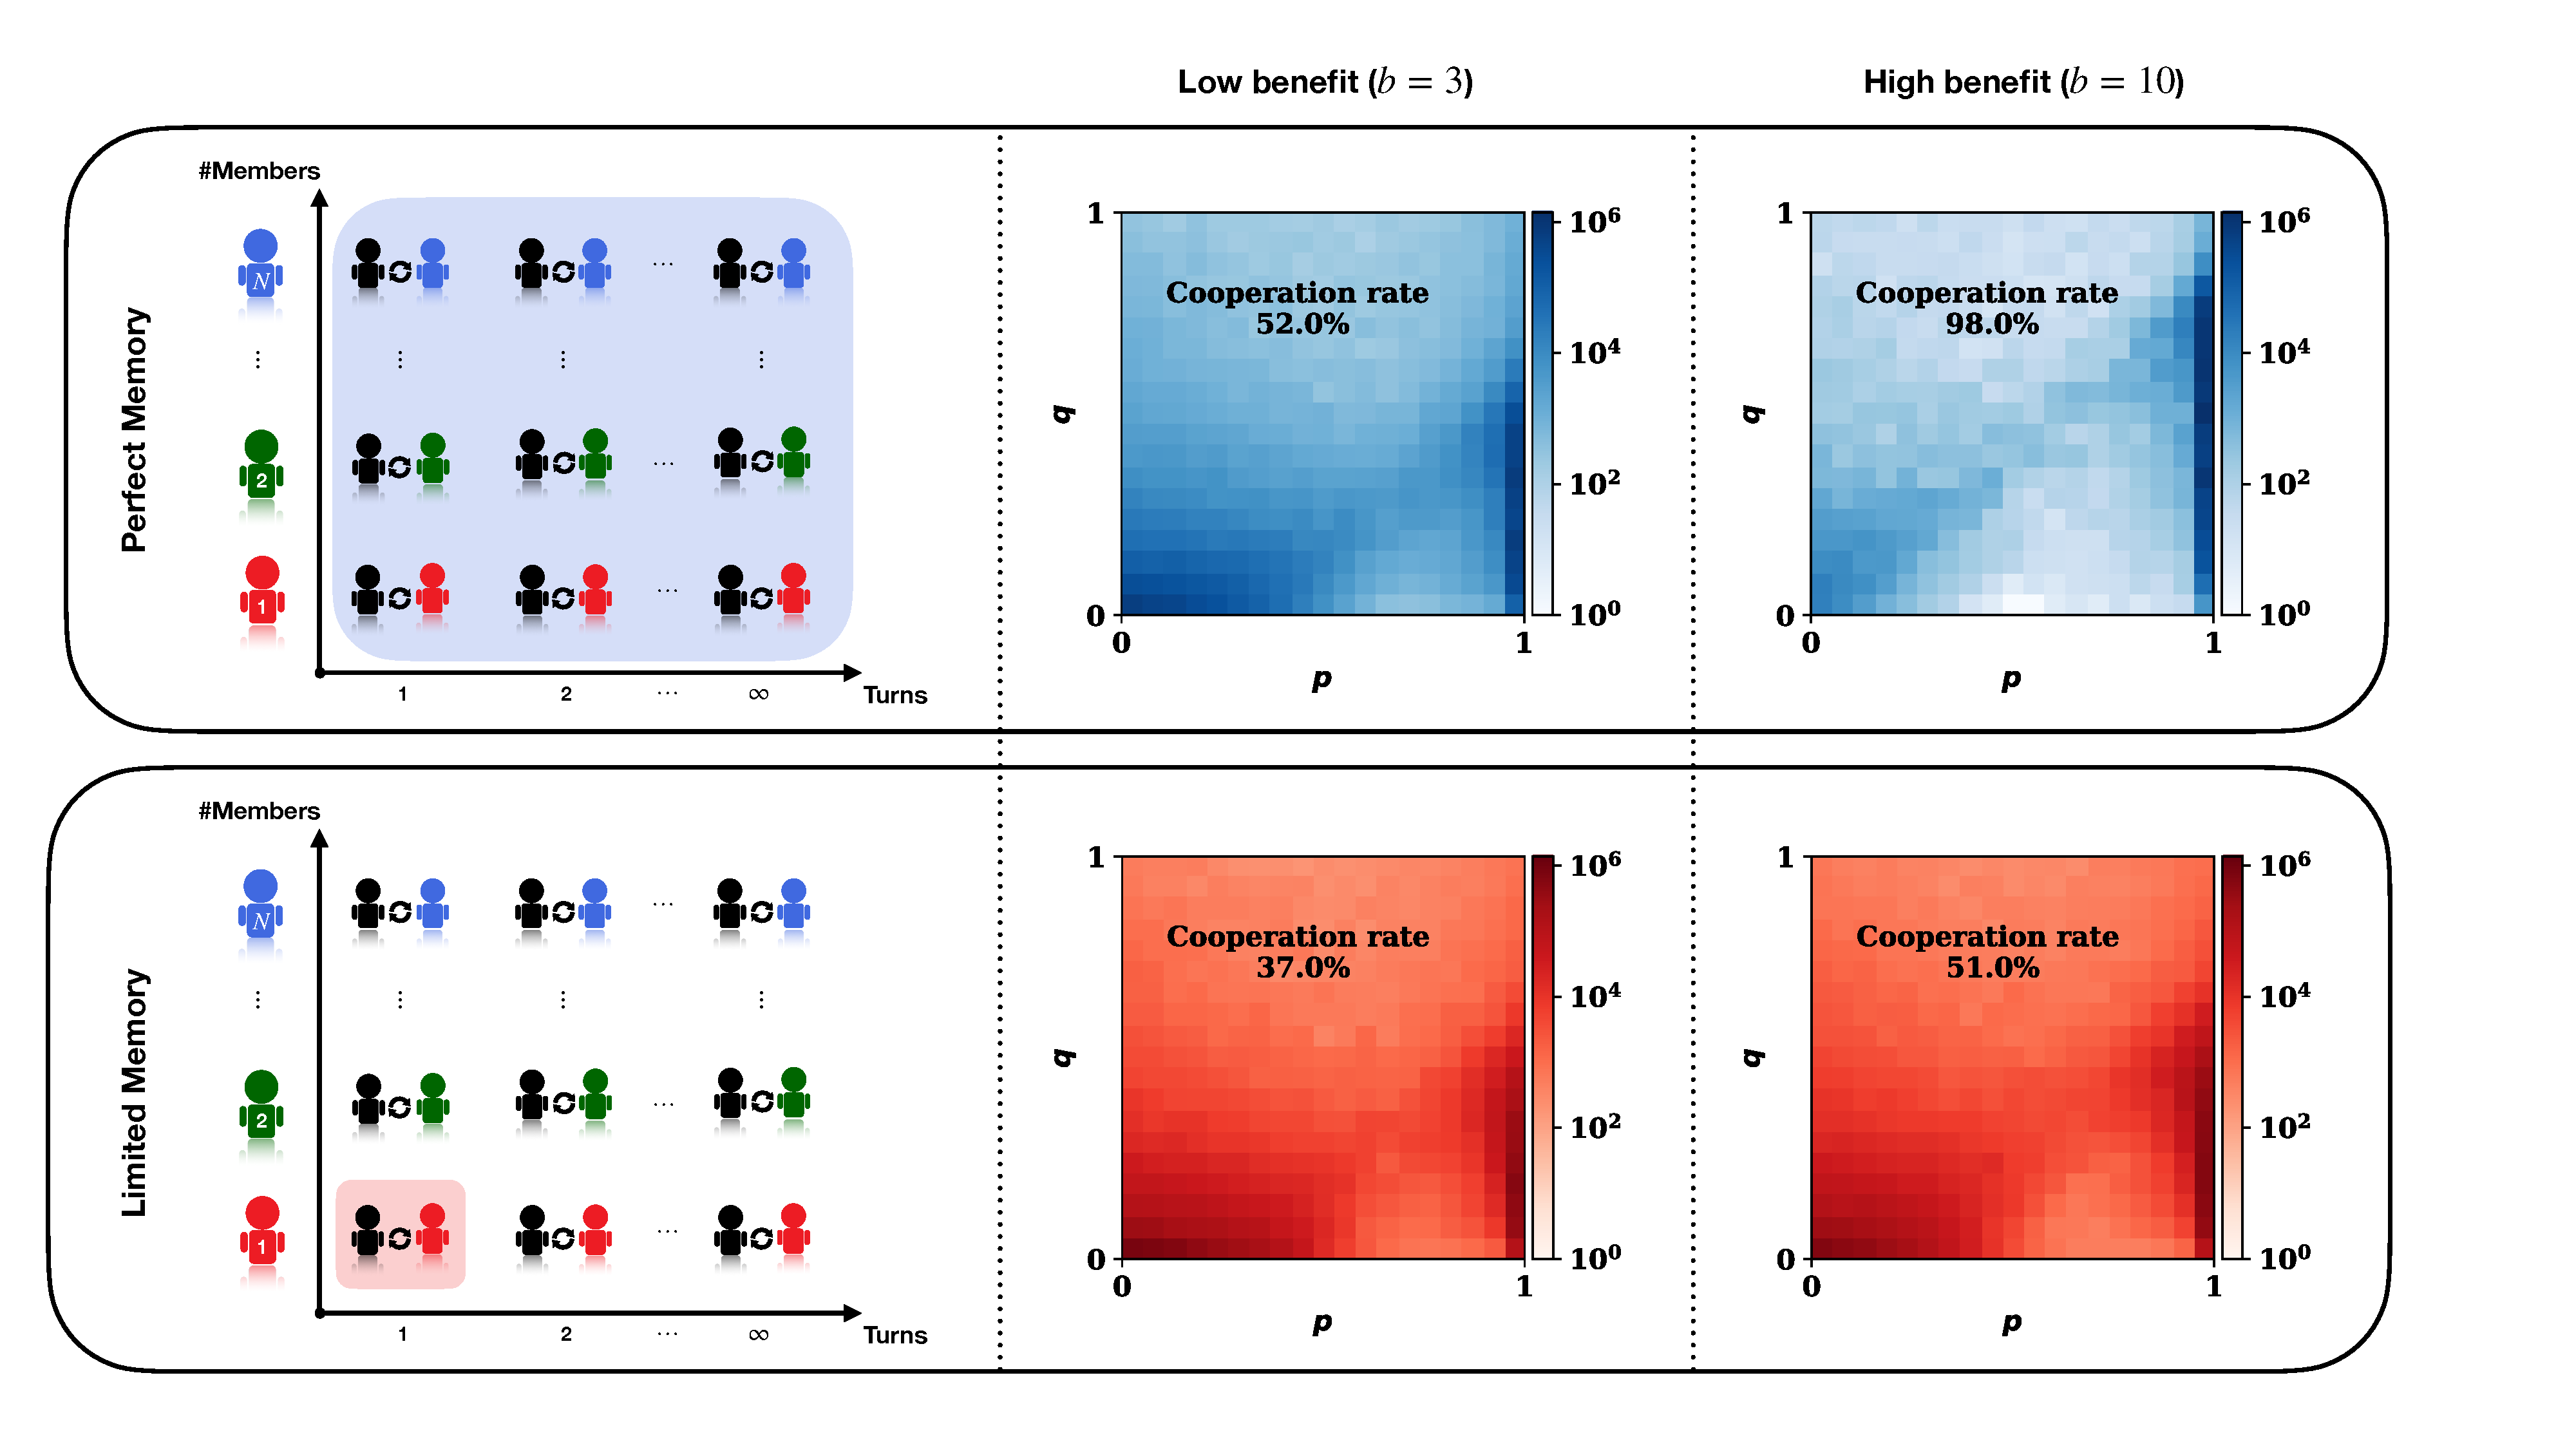
\includegraphics[width=\textwidth]{static/donation_expected_last_round_summary_results.pdf}
    \caption{{\bf Evolutionary dynamics under perfect and limited payoff memory.}
    The leftmost panels give a schematic overview of the two main scenarios we compare. 
    The two scenarios differ in how many past interactions individuals take into account when updating their strategy. 
    In the scenario with perfect payoff memory, individuals consider all their past interactions (against all population members, and taking every turn of each repeated game into account). 
    In the scenario with limited payoff memory, individuals only consider their very last interaction (against one specific population member, taking into account only one round of the repeated game). 
    The four panels  on the right side depict the outcome of evolutionary simulations for repeated games with either a low or a high benefit of cooperation. 
    Colors represent how often the respective region of the strategy space is visited over time. 
    In all four panels, two regions are visited particularly often. 
    One region corresponds to a neighborhood of \alld{} with $p\approx q\!\approx\!0$ (lower left corner). 
    The other region corresponds to a strip of conditionally cooperative strategies with $p\!\approx\! 1$ and $q$ satisfying the constraints \eqref{Eq:PerfectMemory} and \eqref{Eq:LimitedMemory}, respectively (lower right corner). 
    The resulting average cooperation rate depends on which of these two neighborhoods is visited more often. 
    Simulations are run for $T\!=\!10^7$ time steps, using a cost $c\!=\!1$, a continuation probability of $\delta\!=\!0.999$ and a selection strength of $\beta\!=\!1$, in a population of size $N\!=\!100$.}
\label{fig:expected_and_stochastic_for_donation}
\end{figure}


\clearpage
\newpage


\begin{figure}[t]
    \centering
    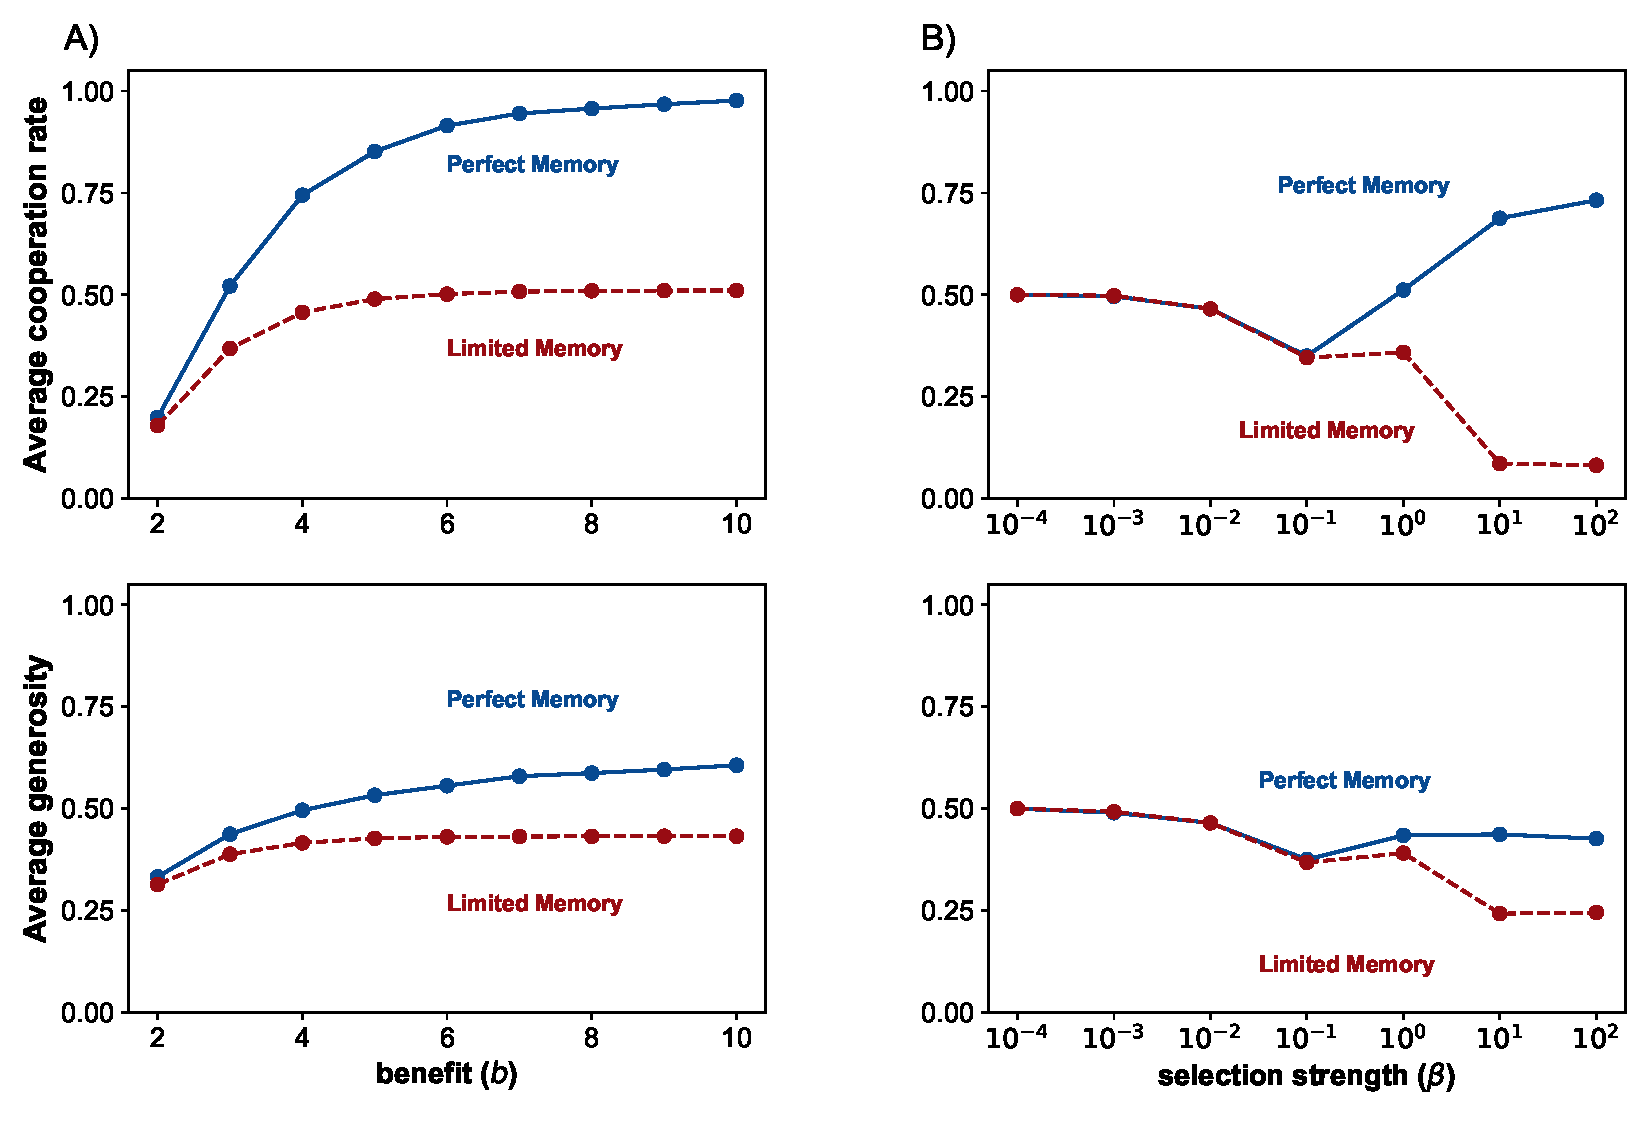
\includegraphics[width=.75\textwidth]{static/cooperation_rate_over_b_and_beta.pdf}
    \caption{{\bf Evolution of direct reciprocity for different parameter values.} 
    To explore the robustness of our results, we have run simulations for different benefit values (left panels, A), and for different selection strengths (right panels, B). 
    In each case, we record the resulting average cooperation rate over the entire simulation (upper panels). 
    In addition we record the individuals' average generosity. 
    Here, we only take into account those residents with $p\! \approx\! 1$ and we compute
    the average of their cooperation probability~$q$. 
    These simulations suggest that perfect payoff memory consistently leads to more cooperation and more generosity. 
    Unless explicitly varied, the parameters of the simulation are $N\!=\!100$, $b\!=\!3$, $c\!=\!1$, $\beta\!=\!1$, $\delta\!=\!0.99$. 
    Simulations are run for $T\!=\!5\times 10^7$ time steps for each parameter combination.}
    \label{fig:cooperation_rate_over_benefit_and_beta}
\end{figure}


\begin{figure}[t]
  \centering
  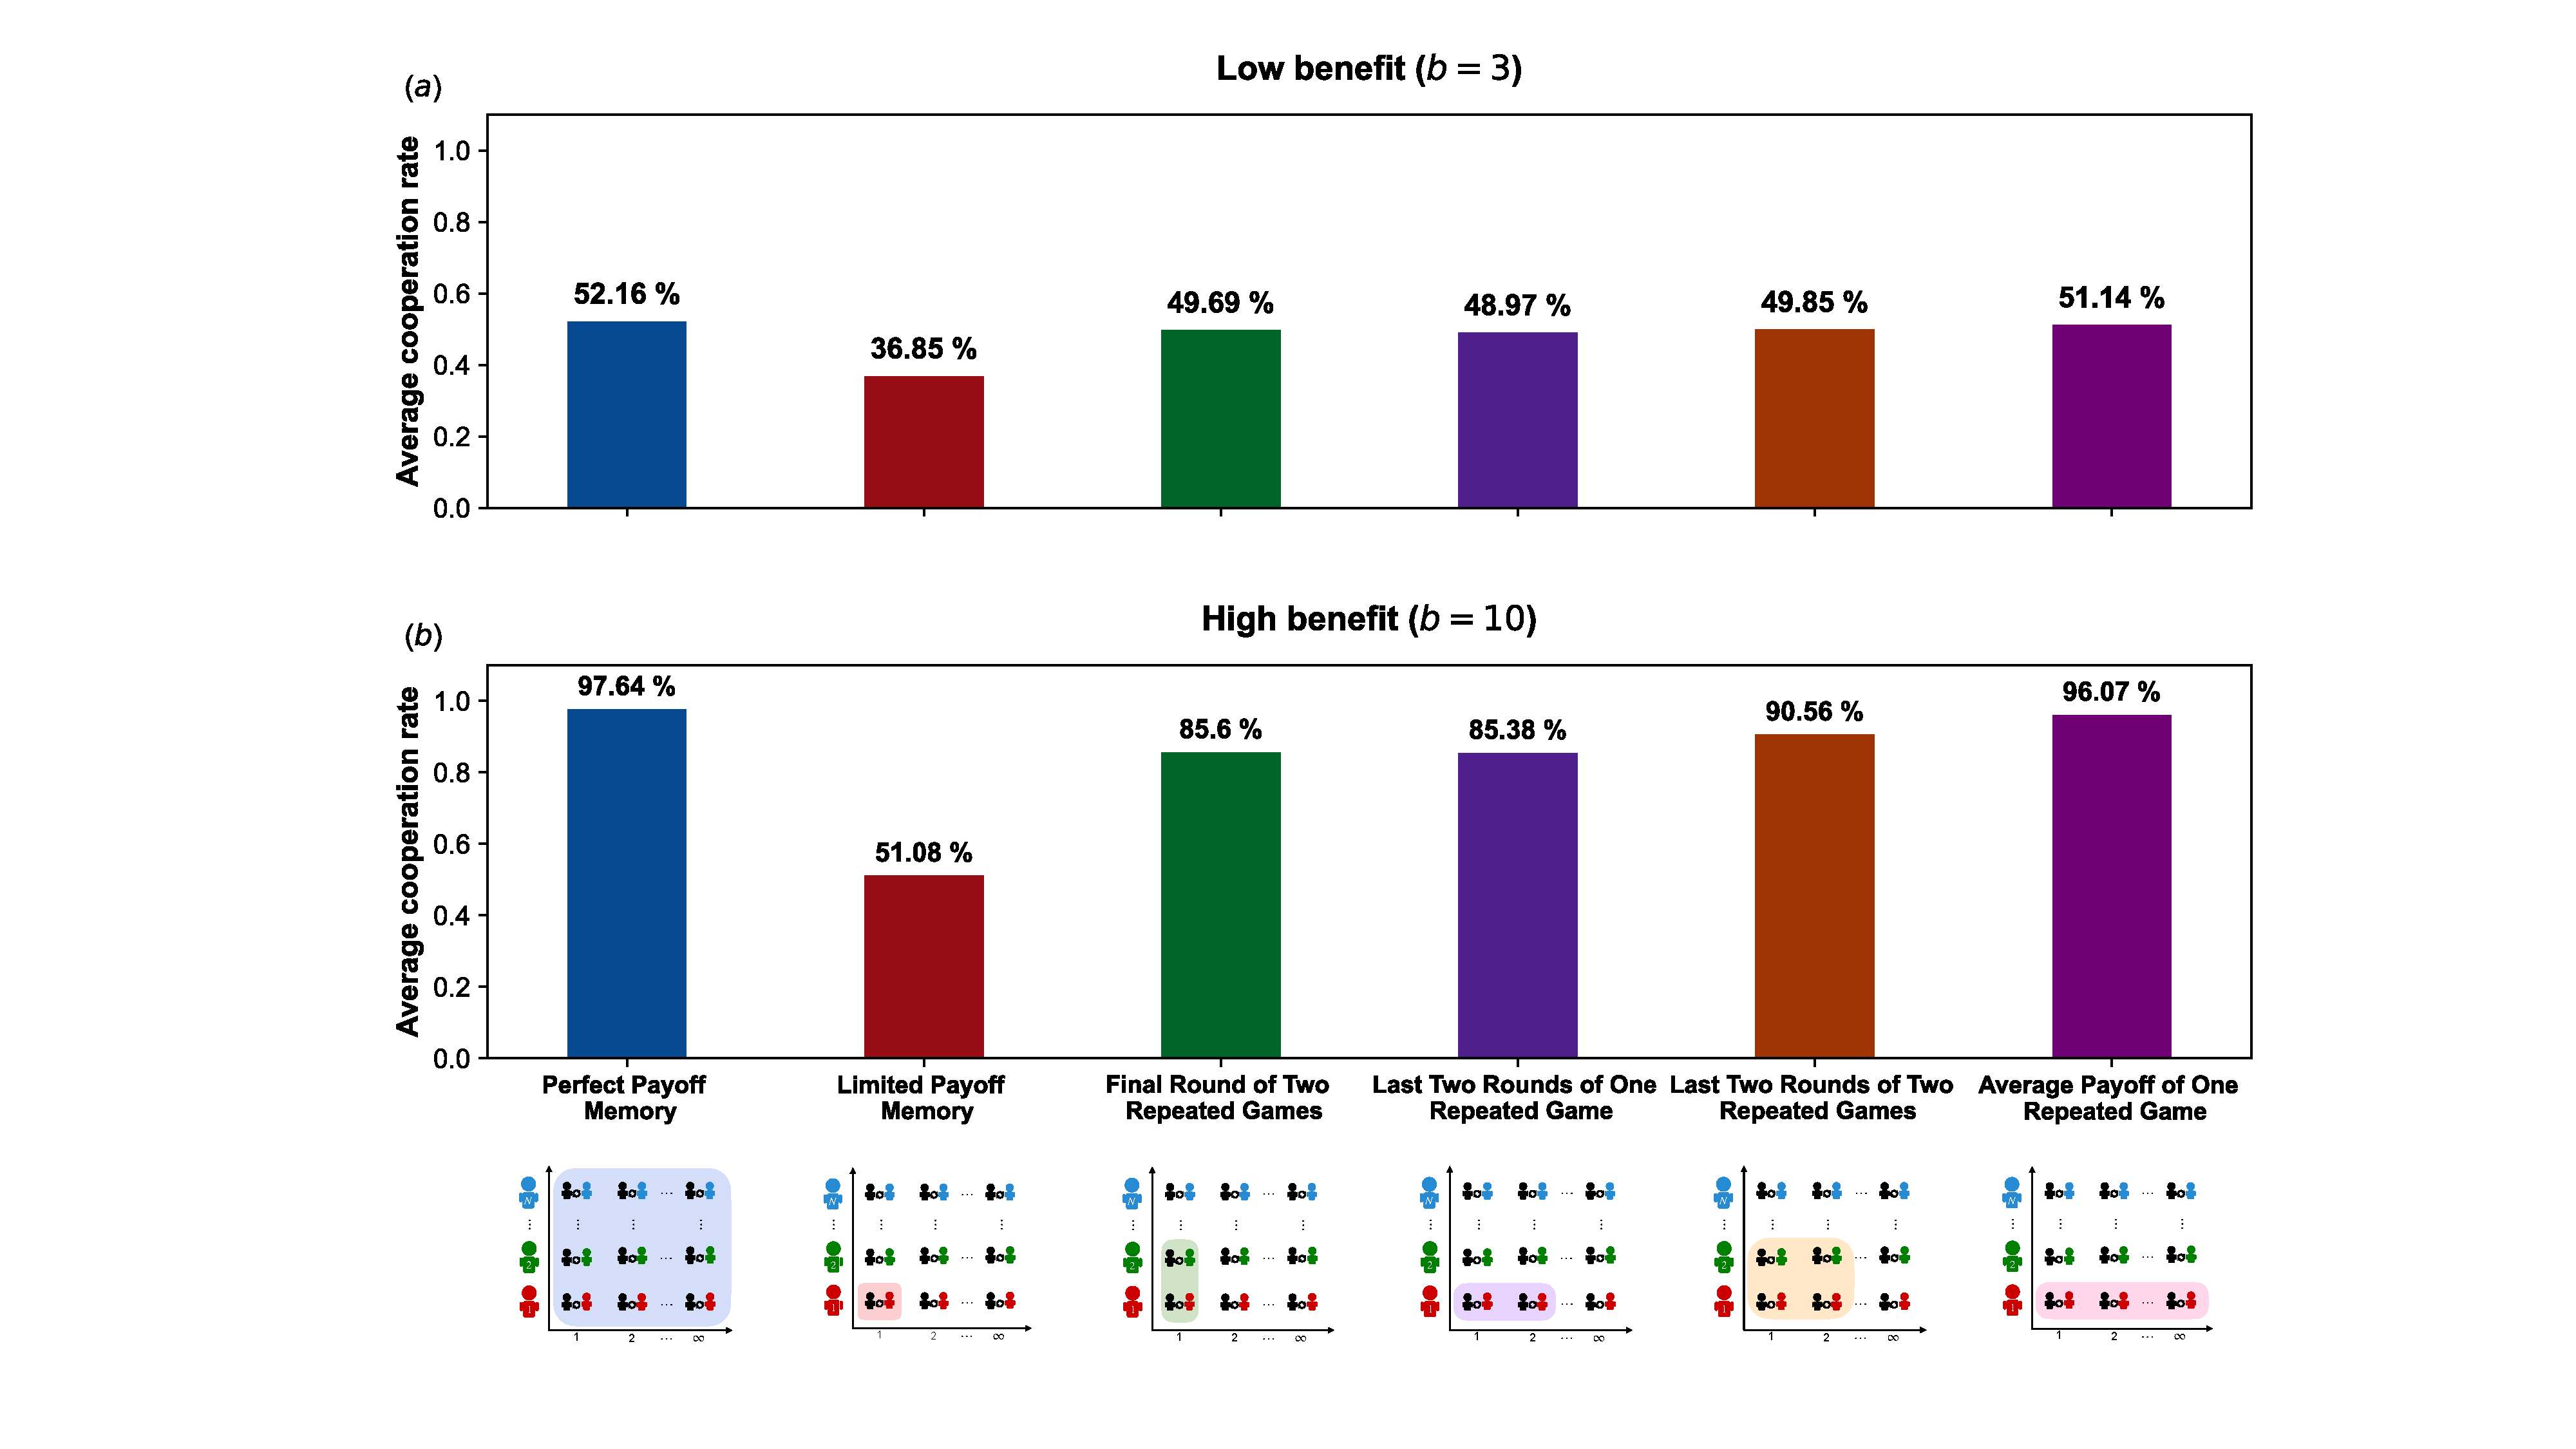
\includegraphics[width=\textwidth]{static/more_memory_summary_results.pdf}
  \caption{{\bf Average cooperation rates for different payoff memories.}
  We vary how much information individuals take into account when updating their strategies. 
  From left to right, we consider the following cases.
  ({\it i}) Updating occurs based on expected payoffs (perfect memory), 
  ({\it ii}) it occurs based on the last round of one interaction (limited memory), 
  ({\it iii}) based on the last round of two interactions,
  ({\it iv}) based on the last two rounds of one interaction, and 
  ({\it v}) based on the last two rounds of two interactions. 
  Again, simulations are run either for a comparably high benefit of cooperation~($b/c\!=\!10$), or for a low benefit~($b/c\!=\!3$). 
  We observe that perfect memory always yields the highest cooperation rate. 
  However, when individuals take into account at least two past interactions -- cases ({\it iii}) to ({\it v}) -- evolving cooperation rates are close to this optimum. 
  Baseline parameters are the same as in \FigDependenceParameters.}
\label{fig:cooperation_rate_all_updating_payoffs}
\end{figure}



\end{document}





%% SOME ADDITIONAL TEXT BITS %%


% repeated game markov chain
given that the opponent cooperated and defected equivalently. The play between a
pair of reactive strategies $s_1 = (y_1, p_1, q_1)$ and $s_2 = (y_2, p_2, q_2)$
can be model as a Markov process with the transition matrix \(M\)~\cite{nowak:APC:1989},

\begin{equation}\label{eq:transition_matrix}
  M = \left[\begin{matrix} p_{1} p_{2} & p_{1} \left(1 - p_{2}\right) & p_{2} \left(1 - p_{1}\right) & \left(1 - p_{1}\right) \left(1 - p_{2}\right)\\
    p_{2} q_{1} & q_{1} \left(1 - p_{2}\right) & p_{2} \left(1 - q_{1}\right) & \left(1 - p_{2}\right) \left(1 - q_{1}\right)\\
    p_{1} q_{2} & p_{1} \left(1 - q_{2}\right) & q_{2} \left(1 - p_{1}\right) & \left(1 - p_{1}\right) \left(1 - q_{2}\right)\\
    q_{1} q_{2} & q_{1} \left(1 - q_{2}\right) & q_{2} \left(1 - q_{1}\right) & \left(1 - q_{1}\right) \left(1 - q_{2}\right)\end{matrix}\right]
\end{equation}

and the stationary vector \(\mathbf{v}(s_1,s_2)\)
which is the solution to \(\mathbf{v}(s_1,s_2) \times M 
= \mathbf{v}(s_1,s_2)\).




% pairwise comparison fixation probability

In fact, so rare that only two different strategies can be
present in the population at any given time. However, in the Supplementary Information
Section 9 we show that the main result holds for \(\mu \neq 0\).
The case of low mutation is vastly adopted because it allows us to explicitly
calculate the fixation probability of a newly introduced mutant. More specifically,
at each step
one individual adopts a mutant strategy randomly selected from the set of
feasible strategies. The fixation probability \(\phi_{M}\) of the mutant
strategy can be calculated explicitly as,

\begin{equation}\label{eq:appendix_fixation_probability}
    \varphi_{M} = \frac{1}{1+\sum\limits_{i=1}^{N-1}\prod\limits_k^i \frac{\lambda^-_k}{\lambda^+_k}},
\end{equation}

where \(k\) is the number of
mutants and \(\lambda^-_k, \lambda^+_k\) are the probabilities that the number of
mutants decreases and increases respectively.
Depending on the fixation probability \(\phi_{M}\) the mutant either
fixes (becomes the new resident) or goes extinct. Regardless, in the next elementary
time step another mutant strategy is introduced to the population. We iterate
this elementary population updating process for a large number of mutant
strategies and we record the resident strategies at each time step. The
probabilities \(\lambda^-_k \text{ and } \lambda^+_k\) depend on the fitness
of the mutant and the resident strategies. In the next section we
present how fitness is calculated in the cases of perfect and limited payoff memory.




% Explicit formulas for the transition probabilities for perfect and limited memory

\subsection{Fitness based on Perfect and Limited Payoff Memory}

In the perfect payoff memory case an individual updates based on the average payoff
against each other member of the population, otherwise known as expected payoffs. 
The payoff of a reactive strategy \(s_1\) against the reactive strategy \(s_2\)
in an infinitely repeated game ($\delta \rightarrow 1$) is explicitly
calculated as,

\[\langle\mathbf{v}(s_1,s_2),\mathbf{u}\rangle.\]

In a population of size \(N\) there are \(k\) mutants and \(N - k\) residents.
Let \(s_M =(y_M, p_M, q_M)\) and \(s_R = (y_R, p_R, q_R)\) denote the
strategies of a mutant and a resident, the expected payoffs \(\pi_R\) and
\(\pi_M\) are given by,

\begin{equation} \label{Eq:ExpPay}
  \begin{array}{lcrcr}
  \displaystyle \pi_R & = &\displaystyle \frac{N\!-\!k\!-\!1}{N-1}\cdot \langle\mathbf{v}(s_R,s_R),\mathbf{u}\rangle	&+	&\displaystyle\frac{k}{N-1}\cdot \langle\mathbf{v}(s_R,s_M),\mathbf{u}\rangle,\\[0.5cm]
  \displaystyle \pi_M & = &\displaystyle\frac{N-k}{N-1}\cdot \langle\mathbf{v}(s_M,s_R),\mathbf{u}\rangle&+	&\displaystyle\frac{k-1}{N-1}\cdot \langle\mathbf{v}(s_M,s_M),\mathbf{u}\rangle.\\
  \end{array}
\end{equation}

The probabilities that the number of mutants decreases and increases,
\(\lambda^-_k\) and \(\lambda^+_k\), in the perfect payoff memory case are
defined as,

\begin{align}\label{eq:perfect_memory_lambdas}
  \lambda^-_k \!=\!\rho(\pi_M, \pi_R) \quad \text{ and } \quad \lambda^+_k \!=\!\rho(\pi_R, \pi_M).
\end{align}

In the case of limited payoff memory we initially define the probability that a
reactive strategy receives the payoff $u\!\in\! \mathcal{U}$ in the very last
round of the game. This is given by Proposition~\ref{proposition:last_round}
(see Supplementary Information Section 2.2.1 for proof).

\begin{Prop}\label{proposition:last_round} Consider a repeated game, with
continuation probability $\delta$, between players with reactive strategies
$s_1\!=\!(y_1, p_1, q_1$)  and $s_2\!=\!(y_2,p_2,q_2)$ respectively. Then
the probability that the $s_1$ player receives the payoff $u\!\in\!
\mathcal{U}$ in the very last round of the game is given by
$v_{u}(s_1,s_2)$, as given by Equation~(\ref{Eq:LastRound}).

\begin{equation} \label{Eq:LastRound}
  \setlength{\arraycolsep}{1pt}
  \begin{array}{rcl}

  v_{r}(s_1,s_2) &= &\displaystyle (1\!-\!\delta)\frac{y_1y_2}{1\!-\!\delta^2 l_1 l_2}+\delta \frac{\Big(q_1+l_1\big((1\!-\!\delta)y_2+\delta q_2\big)\Big) \Big(q_2+l_2\big((1\!-\!\delta)y_1+\delta q_1\big)\Big)}
  {\displaystyle(1\!-\!\delta l_1l_2)(1\!-\!\delta^2 l_1 l_2)},\\[1cm]

  v_{s}(s_1,s_2) &= &\displaystyle (1\!-\!\delta)\frac{y_1\bar{y}_2}{1\!-\!\delta^2 l_1 l_2}+\delta \frac{\Big(q_1+l_1\big((1\!-\!\delta)y_2+\delta q_2\big)\Big) \Big(\bar{q}_2+\bar{r}_2\big((1\!-\!\delta)y_1+\delta p_1\big)\Big)}
  {\displaystyle(1\!-\!\delta l_1l_2)(1\!-\!\delta^2 l_1 l_2)},\\[1cm]

  v_{t}(s_1,s_2) &= &\displaystyle (1\!-\!\delta)\frac{\bar{y}_1y_2}{1\!-\!\delta^2 l_1 l_2}+\delta \frac{\Big(\bar{q}_1+\bar{r}_1\big((1\!-\!\delta)y_2+\delta p_2\big)\Big) \Big(q_2+l_2\big((1\!-\!\delta)y_1+\delta q_1\big)\Big)}
  {\displaystyle(1\!-\!\delta l_1l_2)(1\!-\!\delta^2 l_1 l_2)},\\[1cm]

  v_{p}(s_1,s_2) &= &\displaystyle (1\!-\!\delta)\frac{\bar{y}_1\bar{y}_2}{1\!-\!\delta^2 l_1 l_2}+\delta \frac{\Big(\bar{q}_1+\bar{r}_1\big((1\!-\!\delta)y_2+\delta p_2\big)\Big) \Big(\bar{q}_2+\bar{r}_2\big((1\!-\!\delta)y_1+\delta p_1\big)\Big)}
  {\displaystyle(1\!-\!\delta l_1l_2)(1\!-\!\delta^2 l_1 l_2)}.
  \end{array}
\end{equation}

In these expressions, we have used the notation $l_i:=p_i\!-\!q_i$,
$\bar{y}_i\!=\!1\!-\!y_i$, $\bar{q}_i:=1\!-\!q_i$, and
$\bar{l}_i:=\bar{p}_i\!-\!\bar{q}_i=-l_i$ for $i\!\in\!\{1,2\}$.
\end{Prop}

In the case of limited payoffs memory both the role model and the learner
estimate their fitness after interacting with a single member of the population.
At each time step there are five possible pairings. They interact with each
other with a probability \(\frac{1}{N - 1}\), and they do not interact with
other with a probability \(1 - \frac{1}{N - 1}\). In the latter case, each of
them can interact with either a mutant or a resident. Both of them interact with
a mutant with a probability $\frac{(k-1)(k-2)}{(N-2)(N-3)}$ and both interact
with a resident with a probability $\frac{(N-k-1)(N-k-2)}{(N-2)(N-3)}$. The last
two possible pairings are that either of them interacts with a resident whilst
the other interacts with a mutant, and this happens with a probability
$\frac{(N-k-1)(k-1)}{(N-2)(N-3)}$. We define the probability that the randomly
chosen resident obtained a payoff of $u_R$ in the last round of his respective
game, and that the mutant obtained a payoff of $u_M$ as $x(u_R,u_M)$.

\begin{equation}\label{eq:Chi}
\setlength{\arraycolsep}{1pt}
\begin{array}{llrl}
x(u_R,u_M)	 &=&\displaystyle \frac{1}{N\!-\!1}\cdot  &v_{u_R}(s_R,s_M)\cdot 1_{(u_R,u_M)\in \mathcal{U}^2_F}\\[0.5cm]
&+	
&\displaystyle \left(1\!-\!\frac{1}{N\!-\!1}\right)  
&\left[ \frac{k\!-\!1}{N\!-\!2}\frac{k\!-\!2}{N\!-\!3} v_{u_R}(s_R,s_M) v_{u_M}(s_M,s_M) + 
 \frac{k\!-\!1}{N\!-\!2}\frac{N\!-\!k\!-\!1}{N\!-\!3} v_{u_R}(s_R,s_M) v_{u_M}(s_M,s_R)\right.\\[0.5cm]
&&&\left. +\frac{N\!-\!k\!-\!1}{N\!-\!2}\frac{k\!-\!1}{N\!-\!3} v_{u_R}(s_R,s_R) v_{u_M}(s_M,s_M) + 
 \frac{N\!-\!k\!-\!1}{N\!-\!2}\frac{N\!-\!k\!-\!2}{N\!-\!3} v_{u_R}(s_R,s_R) v_{u_M}(s_M,s_R)\right].
\end{array}
\end{equation}

The probability that the number of mutants increases and decreases by one in the
case of limited payoff memory are now given by,

\begin{align}\label{eq:limited_memory_lambdas}
\lambda^+_k=\frac{N\!-\!k}{N} \cdot \frac{k}{N} \cdot \sum_{u_{R},u_{M}\in\mathcal{U}} x(u_{R},u_{M}) \rho(u_{R},u_{M}) \quad \text{and} \quad
\lambda^-_k=\frac{N\!-\!k}{N} \cdot \frac{k}{N} \cdot \sum_{u_{R},u_{M}\in\mathcal{U}} x(u_{R},u_{M}) \rho(u_{M},u_{R}).
\end{align}

In this expression, $\frac{(N\!-\!k)}{N}$ is the probability that the randomly
chosen learner is a resident, and $\frac{k}{N}$ is the probability that the role
model is a mutant. The sum corresponds to the total probability that the learner
adopts the role model's strategy over all possible payoffs $u_R$ and $u_M$ that
the two player may have received in their respective last rounds.
